%% LyX 2.4.4 created this file.  For more info, see https://www.lyx.org/.
%% Do not edit unless you really know what you are doing.
\documentclass[english,t]{beamer}
\usepackage{mathptmx}
\usepackage[T1]{fontenc}
\usepackage[latin9]{inputenc}
\usepackage{amssymb}
\usepackage{cancel}
\usepackage{graphicx}

\makeatletter

%%%%%%%%%%%%%%%%%%%%%%%%%%%%%% LyX specific LaTeX commands.
%% Because html converters don't know tabularnewline
\providecommand{\tabularnewline}{\\}

%%%%%%%%%%%%%%%%%%%%%%%%%%%%%% Textclass specific LaTeX commands.
% this default might be overridden by plain title style
\newcommand\makebeamertitle{\frame{\maketitle}}%
% (ERT) argument for the TOC
\AtBeginDocument{%
  \let\origtableofcontents=\tableofcontents
  \def\tableofcontents{\@ifnextchar[{\origtableofcontents}{\gobbletableofcontents}}
  \def\gobbletableofcontents#1{\origtableofcontents}
}

%%%%%%%%%%%%%%%%%%%%%%%%%%%%%% User specified LaTeX commands.
\usetheme{Warsaw}
% or ...

\setbeamercovered{transparent}
% or whatever (possibly just delete it)
\setbeamercovered{invisible} %makes overlays invisible

%gets rid of navigation symbols
\setbeamertemplate{navigation symbols}{}

%\usepackage{hyperref}
%\usepackage[usenames,dvipsnames,table]{xcolor} %adds additional color options
\definecolor{links}{HTML}{2A1B81}
%\hypersetup{colorlinks,linkcolor=blue,urlcolor=links}

\usepackage{multicol}

\usepackage{hyperref}

\usepackage{tikz}
\usetikzlibrary{calc}
\usetikzlibrary{plotmarks}
\usetikzlibrary{shapes}
\usepackage{pgfplots} %\usepackage{pgfplots, pgfplotstable}
\pgfplotsset{compat=newest}
\usepackage{filecontents}  %allows in file data
\usepgfplotslibrary{statistics} %allows histogram stuff

\usepackage{forest} %%for tree diagram

\usepackage{calc}
\usepackage[nomessages]{fp}

\usepackage[super]{nth} %easy 1st, 2nd, etc

%\usepackage{advdate}    % Advancing/saving dates
\usepackage{datetime}   % Dates formatting
%\usepackage{datenumber} % Counters for dates

\usepackage[super]{nth}

\usepackage{etex}

\usepackage{fancybox}

%%table colors
%\usepackage[table]{xcolor}
\usepackage{colortbl}

\usepackage[outline]{contour}  %allows text halos

\usepackage{epsdice} %%dice font
\usepackage[misc]{ifsym}
\newfont\dice{dice3d} %%3d dice font

\contourlength{1pt} %sets halo width
%%example: \node at (0.75,0.5) {\contour{white}{\Large Text!}};
%%example:  \node [fill=white,inner sep=1pt] at (2.25,0.5) {\Large 			Text!};
%%example:  \node [fill=white,rounded corners=2pt,inner sep=1pt] at 			(3.75,0.5) {\Large Text!};

%%%%%%%%%%%%%%%%%%%%%%%%%%%
\def\formatdateny{\csname noyear\languagename\expandafter\endcsname\formatdate}
\def\noyearenglish#1, \the\@year{#1}
\let\noyearamerican\noyearenglish
\let\noyearbritish\noyearenglish

%%allows uncover with forest diagrams
\tikzset{
    invisible/.style={opacity=0,text opacity=0},
    visible on/.style={alt=#1{}{invisible}},
    alt/.code args={<#1>#2#3}{%
      \alt<#1>{\pgfkeysalso{#2}}{\pgfkeysalso{#3}} % \pgfkeysalso doesn't change the path
    },
}
\forestset{
  visible on/.style={
    for tree={
      /tikz/visible on={#1},
      edge={/tikz/visible on={#1}}}}}

%%%redefines column alignment to match vertically
%\define@key{beamerframe}{t}[true]{% top
  %\beamer@frametopskip=.2cm plus .5\paperheight\relax%
  %\beamer@framebottomskip=0pt plus 1fill\relax%
 % \beamer@frametopskipautobreak=\beamer@frametopskip\relax%
  %\beamer@framebottomskipautobreak=\beamer@framebottomskip\relax%
  %\def\beamer@initfirstlineunskip{}%
%}

%%provides pdf with 4 slides per page; don't forget to add 'handout' to remove overlays
%\usepackage{pgfpages}
%\pgfpagesuselayout{4 on 1}[a4paper, landscape, border shrink=7mm]
%\pgfpageslogicalpageoptions{1}{border code=\pgfusepath{stroke}}
%\pgfpageslogicalpageoptions{2}{border code=\pgfusepath{stroke}}
%\pgfpageslogicalpageoptions{3}{border code=\pgfusepath{stroke}}
%\pgfpageslogicalpageoptions{4}{border code=\pgfusepath{stroke}}
%%%Don't forget to add 'handout'

\makeatother

\usepackage{babel}
\begin{document}
\newcommand{\gauss}[2]{1/(#2*sqrt(2*pi))*exp(-((x-#1)^2)/(2*#2^2))}

\newcommand{\Gauss}[2]{1/(#2*sqrt(2*pi))*exp(-((x-#1)^2)/(2*#2^2))} %third value is x variable

\newcommand{\xmax}{2000}
\newcommand{\xmin}{0}
\newcommand{\xstep}{0} %must be xmin+n
\newcommand{\ymax}{500}
\newcommand{\ymin}{0}
\newcommand{\ystep}{0} %must be ymin+n

\newcounter{countEx} \setcounter{countEx}{0}
\newcounter{countProb} \setcounter{countProb}{0}
\resetcounteronoverlays{countEx} \resetcounteronoverlays{countProb}

\newcommand{\ex}[3]{
	\addtocounter{countEx}{1}
	\only<#1-#2>{\begin{exampleblock} {Example \chNum.\secNum.\arabic{countEx}.} #3	\end{exampleblock}}
}

\newcommand{\prob}[4]{
	\addtocounter{countProb}{1}
	\only<#1-#2>{\begin{exampleblock} {Problem  \chNum.\secNum.\arabic{countProb}.\,#3} #4	\end{exampleblock}}
}

\newcommand{\yline}[4]{
	(#2 - #4)/(#1 - #3)*(x - #1) + #2
}

\beamerdefaultoverlayspecification{<+->}

%%%%Chapter and Section numbers%%%%%
\newcommand{\chNum}{4}
\newcommand{\secNum}{4}
\newcommand{\secTitle}{Part C: More on Probability and the Standard Distribution}
\date{\formatdate{14}{11}{2014}}

\title[Section \chNum.\secNum: \secTitle]{Section \chNum.\secNum: \secTitle}

\subtitle{Finite Mathematics~~MTH 107~~Fall 2014}

\author{Dr.\,James Ashe}

\titlegraphic{\includegraphics[height=2.75cm]{/home/jim/JamesAshe/MHU/images/MarsHilUniversityLogo-Virtical.png}}

\institute{Mars Hill University}

\makebeamertitle 

%%True false command
\newcommand{\T}{\textcolor{green}{\contour{black}{T}}}
\newcommand{\F}{\textcolor{red}{\contour{black}{F}}}
\newcommand{\uT}[2]{\uncover<#1-#2>{\T}}
\newcommand{\uF}[2]{\uncover<#1-#2>{\F}}

%tkiz ball item 
\newcommand*\circled[1]{\tikz[baseline=(char.base)]
	{\node[circle,ball color=green!50!black!100, shade,   color=white,inner sep=1.2pt] (char) {\tiny #1};
	}
}
\begin{frame}{Schedule}

\begin{center}
\begin{tabular}{|r|l|}
\hline 
\formatdateny{12}{11}{2014} & worksheet 4.4\tabularnewline
\hline 
\formatdateny{14}{11}{2014} & finding values for given probability 4.4\tabularnewline
\hline 
\formatdateny{17}{11}{2014} & more section 4.4 stuff/Review\tabularnewline
\hline 
\formatdateny{19}{11}{2014} & Review\tabularnewline
\hline 
\formatdateny{21}{11}{2014} & \textbf{Exam 4}\tabularnewline
\hline 
\formatdateny{24}{11}{2014} & Review\tabularnewline
\hline 
\formatdateny{26}{11}{2014} & \textbf{Thanksgiving Break}\tabularnewline
\hline 
\formatdateny{28}{11}{2014} & \textbf{Thanksgiving Break}\tabularnewline
\hline 
\formatdateny{1}{12}{2014} & Review\tabularnewline
\hline 
 & \textbf{Final Exam}\tabularnewline
\hline 
\end{tabular}
\par\end{center}

\end{frame}

\begin{frame}{Finding the value from a probability}

\begin{columns}


\column{5.5cm}
\begin{example}
A shoe company collects data and finds that male shoe size is normally
distributed with a mean shoe size of $11$ with a standard deviation
of 1.5. If the company wants to make shoes that will fit 99.7\% of
the male population with sizes centered around the mean, what shoe
sizes should they produce?
\end{example}


\column{5.5cm}
\begin{itemize}
\item <3->[]$11+3\cdot1.5=15.5$
\item <4->[] $11-3\cdot1.5=6.5$
\item <5->[]$p(6.5<x<15.5)$\\
\textrm{$=p(-3<z<3)\approx99.7\%$}
\end{itemize}
\begin{center}
\only<2-4>{\begin{tikzpicture}[scale=.6] 
\begin{axis}[ 
	no markers, 
	domain=0:10, 
	%samples=100, 
	axis lines*=left, 
	xlabel=Standard Distribution, 
	%ylabel=Frequency, 
	height=6cm, %%.6 ratio 
	width=10cm, 
	xtick={-3, -2, -1, 0, 1, 2, 3},
	xticklabels={$\mu-3\sigma$, $\mu-2\sigma$, $\mu-1\sigma$, $\mu$, $\mu+1\sigma$, $\mu+2\sigma$, $\mu+3\sigma$},
	%ytick=empty, 
	enlargelimits=false, 
	clip=false, 
	axis on top, 
	grid = major
	] 
	\addplot [fill=cyan!20, draw, very thick, smooth, domain=-3:3] {\gauss{0}{1}} \closedcycle; 
	\addplot [fill=orange!20, draw=none, domain=-3:-2] {\gauss{0}{1}} \closedcycle; 
	\addplot [fill=orange!20, draw=none, domain=2:3] {\gauss{0}{1}} \closedcycle; 
	\addplot [fill=blue!20, draw=none, domain=-2:-1] {\gauss{0}{1}} \closedcycle; 
	\addplot [fill=blue!20, draw=none, domain=1:2] {\gauss{0}{1}} \closedcycle; 
	\only<1->{
		\node[above] at (axis cs: -0.5, 0.025) {$34.13\%$};} 
	\only<1->{
		\node[above] at (axis cs: 0.5, 0.025) {$34.13\%$};} 
	\only<1->{
		\node[above] at (axis cs: -1.5, 0.025) {$13.59\%$}; 
		\node[above] at (axis cs: 1.5, 0.025) {$13.59\%$};}
	\only<1->{
		\node[above] at (axis cs: 2.5, 0.05) {$2.15\%$}; 
		\node[above] at (axis cs: -2.5, 0.05) {$2.15\%$};}
	\only<1->{ 
		\addplot[<->,black,very thick] coordinates {(-1,0.4) (1,0.4)}; 
		\node[above] at (axis cs: 0, 0.4) {$68.26\%$};} 
	\only<1->{	
		\addplot[<->,black,very thick] coordinates {(-2,0.3) (2,0.3)}; 
		\node[above] at (axis cs: 0, 0.3) {$95.44\%$};}
	\only<1->{
		\addplot[<->,black, very thick] coordinates {(-3,0.2) (3,0.2)}; 
		\node[above] at (axis cs: 0, 0.2) {$99.74\%$};}
	\end{axis} 
\end{tikzpicture}}
\par\end{center}

\begin{center}
\only<5->{\begin{tikzpicture} 
\begin{axis}[ 
	no markers, 
	domain=0:10, 
	%samples=100, 
	axis lines*=left, 
	%xlabel=Standard deviations, 
	%ylabel=Frequency, 
	height=4cm, 
	width=6cm, 
	hide y axis,
	%ticks=none,
	xtick={-3, -2, -1, 0, 1, 2, 3},
	xticklabels={6.5, $$, $$, 11, $$, $$, 15.5},
	%ytick=empty, 
	enlargelimits=false, 
	clip=false, 
	axis on top, 
	%grid = major
	]

	\addplot [fill=blue!50, draw=red,  domain=-3:3] {\gauss{0}{1}} \closedcycle;
		\node[above] at (axis cs: 0.15, 0.05) {$99.7\%$};
	\addplot [draw, thick, smooth, domain=-3.5:3.5] {\gauss{0}{1}} \closedcycle;
	
	%\addplot [fill=orange!20, draw=none, domain=2:3] {\gauss{0}{1}} \closedcycle; 
	%\addplot [fill=blue!20, draw=none, domain=-2:-1] {\gauss{0}{1}} \closedcycle; 
	%\addplot [fill=blue!20, draw=none, domain=1:2] {\gauss{0}{1}} \closedcycle; 
	%\only<1->{\node[above] at (axis cs: -0.5, 0.025) {$34.1\%$};} 
	%\only<1->{\node[above] at (axis cs: 0.5, 0.025) {$34.1\%$};} 
	%\only<1->{\node[above] at (axis cs: -1.5, 0.025) {$13.6\%$};}
	%\only<1->{\node[above] at (axis cs: 1.5, 0.025) {$13.6\%$};}
	%\only<1->{\node[above] at (axis cs: 2.5, 0.05) {$2.1\%$};}
	%\only<1->{\node[above] at (axis cs: -2.5, 0.05) {$2.1\%$};}
	%\only<1->{ \addplot[<->,black,very thick] coordinates {(-1,0.4) (1,0.4)};} 
	%\only<1->{\node[above] at (axis cs: 0, 0.4) {$68.2\%$};} 
	%\only<1->{\addplot[<->,black,very thick] coordinates {(-2,0.3) (2,0.3)};}
	%\only<1->{\node[above] at (axis cs: 0, 0.3) {$95.4\%$};}
	%\only<1->{\addplot[<->,black, very thick] coordinates {(-3,0.2) (3,0.2)};} 
	%\only<1->{\node[above] at (axis cs: 0, 0.2) {$99.7\%$};}
	\end{axis} 
\end{tikzpicture}}
\par\end{center}

\end{columns}
\end{frame}

\begin{frame}{}

\begin{center}
\includegraphics[height=8.5cm]{pics/z-chart-neg-full}
\par\end{center}

\end{frame}

\begin{frame}{}

\begin{center}
\includegraphics[height=8.5cm]{pics/z-chart-pos-full}
\par\end{center}

\end{frame}

\begin{frame}{Finding the value for a probability}

\begin{columns}


\column{5.5cm}
\begin{example}
A shoe company collects data and finds that male shoe size is normally
distributed with a mean shoe size of $11$ with a standard deviation
of 1.5. 

\begin{itemize}
\item [a.] How many \emph{standard deviations} separate the bottom 74.72\%
from the remaining population.
\end{itemize}
\end{example}


\column{5.5cm}
\begin{itemize}
\item <2->[a.]$p(z<c)=74.2\%$
\end{itemize}
\only<3-3>{\includegraphics[width=6cm]{pics/z-chart-65_a}}\only<4-4>{\includegraphics[width=6cm]{pics/z-chart-65_a_box}}\only<5-5>{\includegraphics[width=6cm]{pics/z-chart-65_a_box1}}\only<6-7>{\includegraphics[width=6cm]{pics/z-chart-65_a_box2}}
\begin{itemize}
\item <7->[]$\begin{array}{ccc}
.742 & \rightarrow & .67\\
\mbox{area} &  & z-\mbox{score}
\end{array}$
\item <8->[] $p(z<.67)=74.2$
\end{itemize}
\only<9->{\begin{tikzpicture} 
\begin{axis}[ 
	no markers, 
	domain=0:10, 
	%samples=100, 
	axis lines*=left, 
	%xlabel=Standard deviations, 
	%ylabel=Frequency, 
	height=4cm, 
	width=6cm, 
	hide y axis,
	%ticks=none,
	xtick={-3, -2, -1, 0, 1, 2, 3},
	xticklabels={6.5, 8, 9.5, 11, 12.5, 14, 15.5},
	%ytick=empty, 
	enlargelimits=false, 
	clip=false, 
	axis on top, 
	%grid = major
	]

	\addplot [fill=blue!50, draw=red,  domain=-3.5:.666] {\gauss{0}{1}} \closedcycle;
		\node[above] at (axis cs: 0.15, 0.05) {$99.7\%$};
	\addplot [draw, thick, smooth, domain=-3.5:3.5] {\gauss{0}{1}} \closedcycle;
	
	%\addplot [fill=orange!20, draw=none, domain=2:3] {\gauss{0}{1}} \closedcycle; 
	%\addplot [fill=blue!20, draw=none, domain=-2:-1] {\gauss{0}{1}} \closedcycle; 
	%\addplot [fill=blue!20, draw=none, domain=1:2] {\gauss{0}{1}} \closedcycle; 
	%\only<1->{\node[above] at (axis cs: -0.5, 0.025) {$34.1\%$};} 
	%\only<1->{\node[above] at (axis cs: 0.5, 0.025) {$34.1\%$};} 
	%\only<1->{\node[above] at (axis cs: -1.5, 0.025) {$13.6\%$};}
	%\only<1->{\node[above] at (axis cs: 1.5, 0.025) {$13.6\%$};}
	%\only<1->{\node[above] at (axis cs: 2.5, 0.05) {$2.1\%$};}
	%\only<1->{\node[above] at (axis cs: -2.5, 0.05) {$2.1\%$};}
	%\only<1->{ \addplot[<->,black,very thick] coordinates {(-1,0.4) (1,0.4)};} 
	%\only<1->{\node[above] at (axis cs: 0, 0.4) {$68.2\%$};} 
	%\only<1->{\addplot[<->,black,very thick] coordinates {(-2,0.3) (2,0.3)};}
	%\only<1->{\node[above] at (axis cs: 0, 0.3) {$95.4\%$};}
	%\only<1->{\addplot[<->,black, very thick] coordinates {(-3,0.2) (3,0.2)};} 
	%\only<1->{\node[above] at (axis cs: 0, 0.2) {$99.7\%$};}
	\end{axis} 
\end{tikzpicture}}
\end{columns}
\end{frame}

\begin{frame}{}

\begin{center}
\includegraphics[height=8.5cm]{pics/z-chart-neg-full}
\par\end{center}

\end{frame}

\begin{frame}{}

\begin{center}
\includegraphics[height=8.5cm]{pics/z-chart-pos-full}
\par\end{center}

\end{frame}

\begin{frame}{Finding the value from a probability}

\begin{columns}


\column{5.5cm}
\begin{example}
A shoe company collects data and finds that male shoe size is normally
distributed with a mean shoe size of $11$ with a standard deviation
of 1.5. 

\begin{itemize}
\item [b.] Find the shoe size that separates the bottom $15.15\%$ from
the rest of the population.
\end{itemize}
\end{example}

\begin{block}<4->{Convert \emph{z-}score to data value}
 $c=z\cdot\sigma+\mu$
\end{block}

\column{5.5cm}
\begin{itemize}
\item <2->[b.]$p(x<c)=15.15\%$
\item <3->[]$\begin{array}{ccc}
.1515 & \rightarrow & -1.03\\
\mbox{area} &  & z-\mbox{score}
\end{array}$
\item [] \uncover<5->{\begin{tikzpicture} 
\begin{axis}[ 
	no markers, 
	domain=0:10, 
	%samples=100, 
	axis lines*=left, 
	%xlabel=Standard deviations, 
	%ylabel=Frequency, 
	height=4cm, 
	width=6cm, 
	hide y axis,
	%ticks=none,
	xtick={-3, -2, -1, 0, 1, 2, 3},
	xticklabels={6.5, 8, 9.5, 11, 12.5, 14, 15.5},
	%ytick=empty, 
	enlargelimits=false, 
	clip=false, 
	axis on top, 
	%grid = major
	]

	\addplot [fill=blue!50, draw=red,  domain=-3.5:-1.03] {\gauss{0}{1}} \closedcycle;
		\node[above] at (axis cs: 0.15, 0.05) {$99.7\%$};
	\addplot [draw, thick, smooth, domain=-3.5:3.5] {\gauss{0}{1}} \closedcycle;
	
	%\addplot [fill=orange!20, draw=none, domain=2:3] {\gauss{0}{1}} \closedcycle; 
	%\addplot [fill=blue!20, draw=none, domain=-2:-1] {\gauss{0}{1}} \closedcycle; 
	%\addplot [fill=blue!20, draw=none, domain=1:2] {\gauss{0}{1}} \closedcycle; 
	%\only<1->{\node[above] at (axis cs: -0.5, 0.025) {$34.1\%$};} 
	%\only<1->{\node[above] at (axis cs: 0.5, 0.025) {$34.1\%$};} 
	%\only<1->{\node[above] at (axis cs: -1.5, 0.025) {$13.6\%$};}
	%\only<1->{\node[above] at (axis cs: 1.5, 0.025) {$13.6\%$};}
	%\only<1->{\node[above] at (axis cs: 2.5, 0.05) {$2.1\%$};}
	%\only<1->{\node[above] at (axis cs: -2.5, 0.05) {$2.1\%$};}
	%\only<1->{ \addplot[<->,black,very thick] coordinates {(-1,0.4) (1,0.4)};} 
	%\only<1->{\node[above] at (axis cs: 0, 0.4) {$68.2\%$};} 
	%\only<1->{\addplot[<->,black,very thick] coordinates {(-2,0.3) (2,0.3)};}
	%\only<1->{\node[above] at (axis cs: 0, 0.3) {$95.4\%$};}
	%\only<1->{\addplot[<->,black, very thick] coordinates {(-3,0.2) (3,0.2)};} 
	%\only<1->{\node[above] at (axis cs: 0, 0.2) {$99.7\%$};}
	\end{axis} 
\end{tikzpicture}}
\item <6->[]\only<6-6>{$c=z\cdot\sigma+\mu$}\only<7-7>{$c=(-1.03)\cdot\sigma+\mu$}\only<8-8>{$c=(-1.03)\cdot1.5+11$}\only<9->{$c=9.455$}
\item []$p(x<9.455)=15.15\%$
\end{itemize}
\end{columns}
\end{frame}

\begin{frame}{}

\begin{center}
\includegraphics[height=8.5cm]{pics/z-chart-neg-full}
\par\end{center}

\end{frame}

\begin{frame}{}

\begin{center}
\includegraphics[height=8.5cm]{pics/z-chart-pos-full}
\par\end{center}

\end{frame}

\begin{frame}{Problems}

\prob{1}{1}{The results of a statewide exam for assessing math skills
of realtors was normally distributed with a mean of 72 and a standard
deviation of 12. Those who score in the top 10\% will receive a certificate,
and those who score in the bottom 20\% will be required to attend
a remedial class.}{
\begin{itemize}
\item [a.] What score does a realtor need in order to receive the certificate?
\item [b.] What score will dictate that a realtor must atted the remedial
class?
\end{itemize}
}
\end{frame}

\begin{frame}{Other Fun Stuff}

Often plotted data lies \emph{close }to a line.
\begin{columns}


\column{5.5cm}

\begin{tabular}{|c|c|}
\hline 
\textbf{Hours } & \textbf{Exam }\tabularnewline
\textbf{Studying} & \textbf{Scores}\tabularnewline
\hline 
2 & 55\tabularnewline
\hline 
4 & 70\tabularnewline
\hline 
5 & 64\tabularnewline
\hline 
6 & 80\tabularnewline
\hline 
9 & 87\tabularnewline
\hline 
\end{tabular}
\begin{itemize}
\item <6->We call this a \emph{linear relation. }
\item <7->But which line?
\item <8->We need a reasonable \emph{approximation. }
\end{itemize}

\column{5.5cm}

\vspace{-.5cm}
%%%%%%%
\begin{tikzpicture} 
\begin{axis}[height=5.5cm, 
	width=5.5cm, axis lines=middle,
	minor x tick num={4},minor y tick num={4},
	grid=both,
	xmin=0,
	xmax=10,
	ymin=50,
	ymax=100,
	xlabel={$Hours$},ylabel={$Scores$}, 
	%xtick={0,50,...,250},%ytick={0,10,20,...,40},%axis line style={-latex},
	every axis/.append style={font=\footnotesize},
	%restrict y to domain=-1:10,%no markers, 
	%every axis x label/.append style={anchor=north},%every axis y label/.append style={anchor=east}
	/pgf/number format/1000 sep={}
	]
  
	\only<2->{\addplot[draw=none,color=blue,solid,mark=*,style={font=\footnotesize}] coordinates {(2,55) (4,70) (5,64) (6,80) (9,87)};}
	
	\only<3->{\addplot[thick,draw=red,domain=0:10]{\yline{2}{55}{6}{80}} node[pos=.65,above] {$$};}
	\only<3->{\addplot[draw=none,color=red,solid,mark=*,style={font=\footnotesize}] coordinates {(2,55)  (6,80)};}

	\only<4->{\addplot[thick,draw=blue,domain=0:10]{\yline{6}{80}{9}{87}} node[pos=.65,above] {$$};}
	\only<4->{\addplot[draw=none,color=blue,solid,mark=*,style={font=\footnotesize}] coordinates {(6,80)  (9,87)};}

	\only<5->{\addplot[thick,draw=purple,domain=0:10]{\yline{4}{70}{9}{87}} node[pos=.65,above] {$$};}
	\only<5->{\addplot[draw=none,color=purple,solid,mark=*,style={font=\footnotesize}] coordinates {(4,70)  (9,87)};}
	
\end{axis}
\end{tikzpicture}
\end{columns}
\end{frame}

\begin{frame}{The Least Squares Line (``best-fit line'')}

\begin{columns}


\column{5.5cm}

\begin{tabular}{|c|c|}
\hline 
\textbf{Hours } & \textbf{Exam }\tabularnewline
\textbf{Studying} & \textbf{Scores}\tabularnewline
\hline 
2 & 55\tabularnewline
\hline 
4 & 70\tabularnewline
\hline 
5 & 64\tabularnewline
\hline 
6 & 80\tabularnewline
\hline 
9 & 87\tabularnewline
\hline 
\end{tabular}

\column{5.5cm}
\begin{block}<2->{Least Square Line \emph{slope}}
$m=\frac{n(\sum xy)-(\sum x)(\sum y)}{n(\sum x^{2})-(\sum x)^{2}}$
\end{block}
\vspace{0cm}
\begin{block}<3->{Least Square Line \emph{y-int}}
$b=\frac{\sum y-m(\sum x)}{n}$
\end{block}
\vspace{0cm}
\begin{block}<4->{Least Square Line}
$y=mx+b$
\end{block}
\end{columns}
\end{frame}

\begin{frame}{}

\begin{columns}


\column{5.5cm}

\begin{tabular}{|c|c|}
\hline 
\textbf{Hours } & \textbf{Exam }\tabularnewline
\textbf{Studying} & \textbf{Scores}\tabularnewline
\hline 
2 & 55\tabularnewline
\hline 
4 & 70\tabularnewline
\hline 
5 & 64\tabularnewline
\hline 
6 & 80\tabularnewline
\hline 
9 & 87\tabularnewline
\hline 
\end{tabular}
\begin{exampleblock}{Equation of the least squares line}
$y=(4.54)x+47.57$
\end{exampleblock}
\begin{block}<2->{Correlation Coefficient}
$r=\frac{n(\sum xy)-(\sum x)(\sum y)}{\sqrt{n(\sum x^{2})-(\sum x)^{2}}\sqrt{n(\sum y^{2})-(\sum y)^{2}}}$
\end{block}


\column{5.5cm}

\vspace{-.5cm}
%%%%%%%
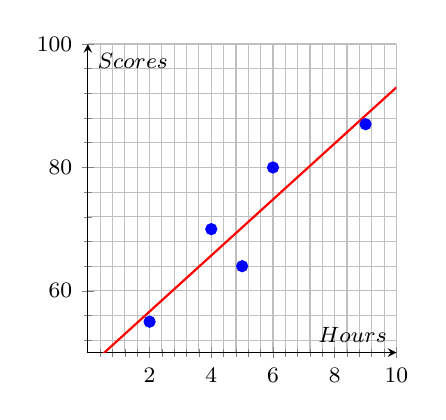
\begin{tikzpicture} 
\begin{axis}[height=5.5cm, 
	width=5.5cm, axis lines=middle,
	minor x tick num={4},minor y tick num={4},
	grid=both,
	xmin=0,
	xmax=10,
	ymin=50,
	ymax=100,
	xlabel={$Hours$},ylabel={$Scores$}, 
	%xtick={0,50,...,250},%ytick={0,10,20,...,40},%axis line style={-latex},
	every axis/.append style={font=\footnotesize},
	%restrict y to domain=-1:10,%no markers, 
	%every axis x label/.append style={anchor=north},%every axis y label/.append style={anchor=east}
	/pgf/number format/1000 sep={}
	]
  
	\only<2->{\addplot[draw=none,color=blue,solid,mark=*,style={font=\footnotesize}] coordinates {(2,55) (4,70) (5,64) (6,80) (9,87)};}
	
	\only<2->{\addplot[thick,draw=red,domain=0:10]{4.54*x+47.57} node[pos=.65,above] {$$};}
	
\end{axis}
\end{tikzpicture}
\end{columns}
\end{frame}

\begin{frame}{}

\prob{1}{}{Find the equation of the least squares line.}{The paired data below consist of the costs of advertising (in thousands) and the number of products sold (in thousands).}

\footnotesize{%
\begin{tabular}{c|c|c|c|c|c|c|c|c}
Cost(\emph{x}) & 9 & 2 & 3 & 4 & 2 & 5 & 9 & 10\tabularnewline
\hline 
Number(\emph{y}) & 85 & 52 & 55 & 68 & 67 & 86 & 83 & 73\tabularnewline
\end{tabular}}

.
\begin{columns}


\column{5.5cm}
\begin{itemize}
\item <3->[]\large$y=2.79x+55.8$
\item <4->[]$r\approx.708$
\end{itemize}

\column{5.5cm}

\vspace{-.5cm}
%%%%%%%
\begin{tikzpicture} 
\begin{axis}[height=5.5cm, 
	width=5.5cm, axis lines=middle,
	minor x tick num={4},minor y tick num={4},
	grid=both,
	xmin=0,
	xmax=11,
	ymin=50,
	ymax=90,
	xlabel={$Cost$},ylabel={$Number$}, 
	%xtick={0,50,...,250},%ytick={0,10,20,...,40},%axis line style={-latex},
	every axis/.append style={font=\footnotesize},
	%restrict y to domain=-1:10,%no markers, 
	%every axis x label/.append style={anchor=north},%every axis y label/.append style={anchor=east}
	/pgf/number format/1000 sep={}
	]
  
	\only<2->{\addplot[draw=none,color=blue,solid,mark=*,style={font=\footnotesize}] coordinates {(9,85) (2,52) (3,55) (4,68) (2,67) (5,86) (9,85) (10,73)};}
	\only<3->{\addplot[thick,draw=red,domain=0:11]{2.79*x+55.8} node[pos=.65,above] {$$};}
	

\end{axis}
\end{tikzpicture}
\end{columns}
\end{frame}

\begin{frame}{Other Fun Stuff}

\begin{columns}


\column{5.5cm}
\begin{itemize}
\item []\textbf{ Margin of Error}
\item <2->A poll of $30$ people is taken.
\item <3->Thre are many ways to select $30$ people from the population.
\item <4->The set of all possible polls is also a population with its own
$\mu$ and $\sigma$.
\item <5->By the \emph{Central Limit Theorem}, any population of samples
is normally distributed for large enough samples.
\item []<6->($n=30$ is large enough)
\item <7->$5\%$ chance a randomly selected poll is within $2\cdot\sigma$
of the actual result. 
\end{itemize}

\column{5.5cm }
\begin{itemize}
\item [] \uncover<8->{\begin{tikzpicture} 
\begin{axis}[ 
	no markers, 
	domain=0:10, 
	%samples=100, 
	axis lines*=left, 
	%xlabel=Standard deviations, 
	%ylabel=Frequency, 
	height=4cm, 
	width=6cm, 
	hide y axis,
	%ticks=none,
	xtick={-3, -2, -1, 0, 1, 2, 3},
	xticklabels={$$, $-2 \sigma$,$$,$$, $$, $2 \sigma$,},
	%ytick=empty, 
	enlargelimits=false, 
	clip=false, 
	axis on top, 
	%grid = major
	]

	\addplot [fill=red!50, draw=red,  domain=-3.5:-2] {\gauss{0}{1}} \closedcycle;
	\addplot [fill=red!50, draw=red,  domain=2:3.5] {\gauss{0}{1}} \closedcycle;
		%\node[above] at (axis cs: 0.15, 0.05) {$99.7\%$};
	\addplot [draw, thick, smooth, domain=-3.5:3.5] {\gauss{0}{1}} \closedcycle;
	
	%\addplot [fill=orange!20, draw=none, domain=2:3] {\gauss{0}{1}} \closedcycle; 
	%\addplot [fill=blue!20, draw=none, domain=-2:-1] {\gauss{0}{1}} \closedcycle; 
	%\addplot [fill=blue!20, draw=none, domain=1:2] {\gauss{0}{1}} \closedcycle; 
	%\only<1->{\node[above] at (axis cs: -0.5, 0.025) {$34.1\%$};} 
	%\only<1->{\node[above] at (axis cs: 0.5, 0.025) {$34.1\%$};} 
	%\only<1->{\node[above] at (axis cs: -1.5, 0.025) {$13.6\%$};}
	%\only<1->{\node[above] at (axis cs: 1.5, 0.025) {$13.6\%$};}
	%\only<1->{\node[above] at (axis cs: 2.5, 0.05) {$2.1\%$};}
	%\only<1->{\node[above] at (axis cs: -2.5, 0.05) {$2.1\%$};}
	%\only<1->{ \addplot[<->,black,very thick] coordinates {(-1,0.4) (1,0.4)};} 
	%\only<1->{\node[above] at (axis cs: 0, 0.4) {$68.2\%$};} 
	%\only<1->{\addplot[<->,black,very thick] coordinates {(-2,0.3) (2,0.3)};}
	%\only<1->{\node[above] at (axis cs: 0, 0.3) {$95.4\%$};}
	%\only<1->{\addplot[<->,black, very thick] coordinates {(-3,0.2) (3,0.2)};} 
	%\only<1->{\node[above] at (axis cs: 0, 0.2) {$99.7\%$};}
	\end{axis} 
\end{tikzpicture}}
\end{itemize}
\end{columns}
\end{frame}

\end{document}
